%!TEX root = ../thesis.tex
\subsection{基因演算法架構及求解}
\label{c:ch6.3.2}
從上一章節介紹了基因演算法的核心概念後,本章將介紹典型基因演算法的演算流程,如圖\ref{fig:flow4}所表示
\begin{figure}[!htb]
\center
%!TEX root = ../thesis.tex
\tikzstyle{endpoint} = [rectangle,draw,rounded corners, minimum width=7em, minimum height=2em,text centered, draw=black]
\tikzstyle{decision} = [diamond, draw, 
    text width=5em, text badly centered, node distance=3cm, inner sep=0pt]
\tikzstyle{block} = [rectangle, draw, 
    text width=7em, text centered, minimum height=2em]
\tikzstyle{line} = [draw, -latex']
    
\begin{tikzpicture}[node distance = 1.5cm, auto]
    % Place nodes
    \node [endpoint] (init) {隨機產生染色體};
    \node [block, below of=init] (fitness) {計算適應函數};
    \node [decision, below of=fitness] (decide) {是否滿足終止條件};
    \node [endpoint, below of=decide,node distance=3cm] (sol) {求得最佳解};
    \node [block, right of=decide,node distance=4cm] (reprod) {複製};
    \node [block, below of=reprod] (cross) {交配};
    \node [block, below of=cross] (mutate) {突變};
    % Draw edges
    \path [line] (init) -- (fitness);
    \path [line] (fitness) -- (decide);
    \path [line] (decide) -- node {Yes}(sol);
    \path [line] (decide) -- node {No}(reprod);
    \path [line] (reprod) -- (cross);
    \path [line] (cross) -- (mutate);
    \draw [line] (mutate) -- +(2,0) -- +(2,6) -- +(-2.4,6);
\end{tikzpicture}
\caption{基因演算法流程圖}
\label{fig:flow4}
\end{figure}
我們將從圖\ref{fig:flow4}逐步介紹基因演算流程圖
\begin{enumerate}[]
\item \textbf{隨機產生染色體:}\\
染色體(chromosome)代表一組可行解,在本研究當中為各個染整製程因子的組合,而在選定起始解當時通常我們會隨機的選定五個因子的值。
\item \textbf{產生適應函數:}\\
適應函數(fitness function)通常代表每一組染色體的優劣程度依據,在本研究當中目標函式就是每一組染整製程是否好壞的依據。
\item \textbf{滿足終止條件:}\\
終止條件通常會設定固定的遺傳代次(generation times),當到達迭代的次數則演算停止,以目前的結果作為最佳解,或者設定此次的最佳解與前一次的最佳解之間的誤差不超過某個微小值,為演算停止條件。
\item \textbf{複製:}\\
複製的過程當通常會選擇適應函數結果較好的染色體作為複製的對象,在本研究當中主要都以最小化作為搜尋的方向,故會挑選適應函數較小者為複製對象。
\item \textbf{交配:}\\
會從當代的染色體兩兩互相生成下一代的染色體稱為交配行為,而在交配過程當中會在當代的兩個染色體互相交換部份因子結果,例如在本研究當中會交換兩組參數因子中的前兩個因子,作為下一代次的染色體。
\item \textbf{突變:}\\
會在當代的染色體中機率性的選擇染色體內的某些組合因子,進行數值的變化,而在本研究當中為了不讓其搜尋過程容易掉入區域最佳解當中,會機率性的對五個因子做數值的變化,以增加搜索的可能性。
\end{enumerate}

在瞭解基因演算法基本架構後,我們將從\cite{Wu.etc}所使用的基因演算法,搜尋本研究所設置的三個主要的模型的最佳解,不過在求解之前由於前面章節提到,評判染色體的優劣主要依據適應函式的值,但在模型當中還需要考慮限制條件,而\cite{Wu.etc}使用Penalty方法,將限制式轉化為懲罰函式再將它併入目標函式,讓適應函式同時擁有目標函式以及限制的資訊,如\ref{eq:fitness}式,其中的Penalty函式$p(x)$在可行解時則懲罰值為0,反之則為懲罰函數值,$\Delta b(x)$為超出限制範圍的限制式,而$\Delta b^{nef}(x)$為接近可行解的閥值,如\ref{eq:penalty}式
\begin{equation}
F(x)=f(x)+p(x)
\label{eq:fitness}
\end{equation}
\begin{equation}
p(x)=
	\begin{cases}
	0,x\in feasible\ solution\\
	\sum_{i}^{m} \bigl(\frac{(\Delta b_{i}(x))}{\Delta b_{i}^{nef}(x)}\bigr)^{2}\\
	\end{cases}
\label{eq:penalty}
\end{equation}
在設定適應函式後,我們選擇\cite{rainville2012deap}中所提到的開放式資源,由於使用上較為穩定,且容易取得及使用,因此將套用python的Deap套件裡的基因演算方法求解,並根據\cite{Wu.etc}中的設定,將交配比率設為四分之一以及突變率設定為0.2,每一個代次染色體數設定為300個,並將迭代次數設定為500次,由演算過後如圖\ref{fig:GAopt}為三個主要模型各自的收斂狀況圖
\begin{figure}[!htb]
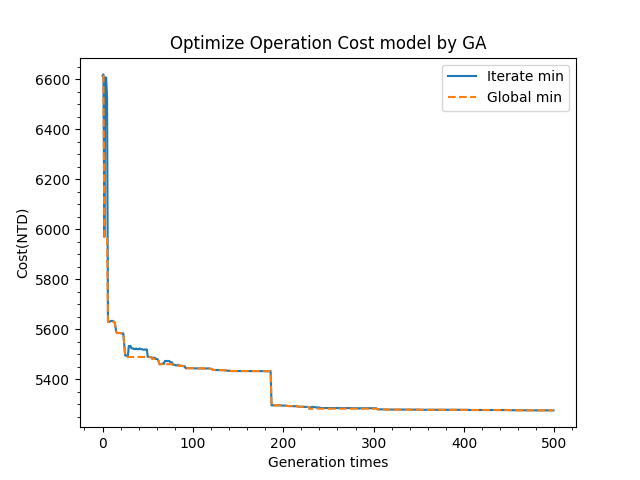
\includegraphics[width=8cm,height=6cm]{Graph/GAcost.png}
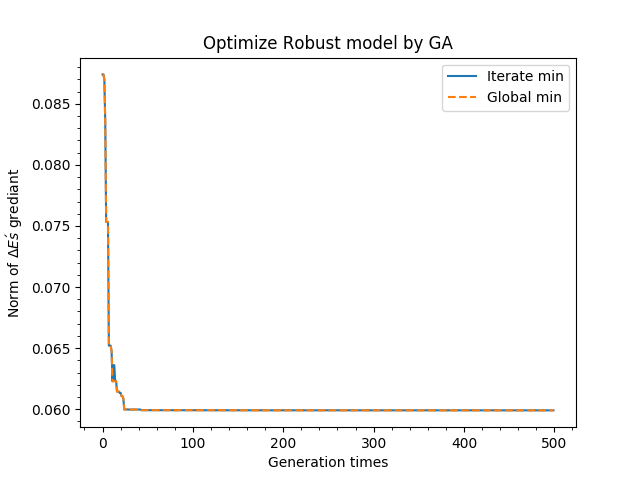
\includegraphics[width=8cm,height=6cm]{Graph/GARobust.png}
\center
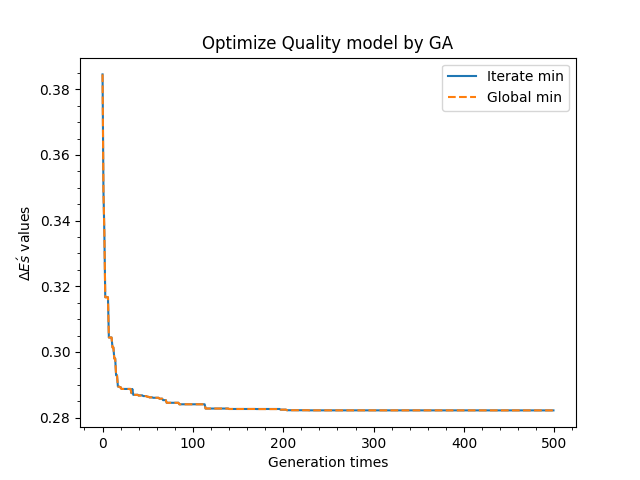
\includegraphics[width=8cm,height=6cm]{Graph/GADeltaE.png}
\caption{GA演算法搜尋各個模型最佳化收斂過程圖}
\label{fig:GAopt}
\end{figure}
\\由圖\ref{fig:GAopt}(左上)以GA演算法求解運作成本最小化模型,成本最佳解可以達到5275元,圖\ref{fig:GAopt}(右上)以GA演算法求解穩定度模型,其最佳解可達到約0.06,而圖\ref{fig:GAopt}(下)為品質成本的收斂過程圖,其$\Delta E$可達0.28,為了將得到的結果調整為符合實際紡織產業所能控制的範疇,如表\ref{tab:table7}將各個搜尋結果調整後分別套用至每個目標函數,便可比較製程參數組合間的差異。
\begin{table}[!htbp]
	\caption{基因演算法模型最佳化結果表}
	\center
	%!TEX root = ../thesis.tex
\begin{tabular}{ccccccccc}
\hline
\multirow{2}{*}{Items} &
\multicolumn{5}{c}{Factors} &
\multicolumn{3}{c}{\multirow{1}{*}{Result}} \\
\cline{2-9}
  & $x_A$ & $x_B$ & $x_C$ & $x_D$ & $x_E$ & Cost & Robust & $\Delta E$ \\
\hline\hline
最小化成本 & 51 & 1.3 & 76 & 18 & 15 & 5368 & 0.49 & 0.63 \\ 
穩定度最佳化 & 59 & 1.2 & 86 & 19 & 20 & 6590 & 0.065 & 0.168 \\ 
品質最佳化 & 61 & 1.2 & 82 & 19 & 23 & 7163 & 0.115 & 0.086 \\ 
\hline
\end{tabular}
	\label{tab:table7}
\end{table}




